\documentclass[preview=true]{standalone}
\usepackage{tikz}
\usepackage{pgfplots}
\usepackage[siunitx, american]{circuitikz}
\usepackage[utf8]{inputenc}
\usepackage{newtxtext,newtxmath}
\usepackage[T1]{fontenc}
\pgfplotsset{compat=1.18}
\usepgfplotslibrary{units, fillbetween, smithchart, colormaps}
\usetikzlibrary{positioning, shapes, arrows, arrows.meta, graphs, shapes.geometric, math}
\tikzset{>=latex} % Better arrow tips

\begin{document}
    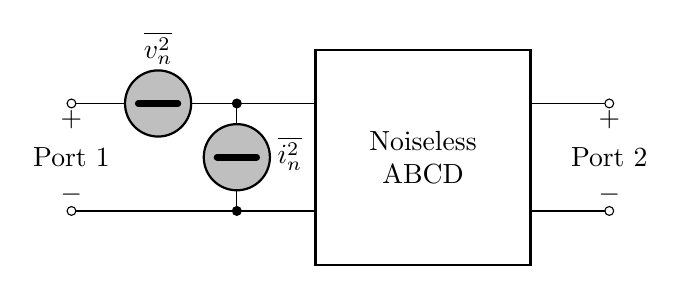
\begin{tikzpicture}
    \draw 
    node[fourport, align=center, scale=1.5] (z1) {} 
    (z1.port4) to[short, -*] ++(-1,0) coordinate (Z1A)
    (z1.port3) to[short, -o] ++(1,0) coordinate (Z1B)
    (z1.port2) to[short, -o] ++(1,0) coordinate (Z1C)
    (z1.port1) to[short, -*] ++(-1,0) coordinate (Z1D)

    (Z1A) to[noise current source, l^={$\overline{i_n^2}$}] (Z1D)
    (Z1A) to[noise voltage source, l_={$\overline{v_n^2}$}] ++(-2,0) to [short,-o] ++(-0.1,0) coordinate (in_p)
    (Z1D) to [short, -o] ++(-2.1,0) coordinate (in_n)

    (in_p) to [open, v^>=Port 1] (in_n)
    (Z1B) to [open, v^>=Port 2] (Z1C)
    
    ;
    \node[align=center] at (z1) {Noiseless \\ ABCD};
    \end{tikzpicture}
\end{document}